% Analisi dei requisiti

\chapter{Analisi dei requisiti}

% TODO: CTO e CEO in glossary?
% TODO: feature in glossary?
% TODO: beta tester in glossary?
PastBot nasce da un insieme di nuove tecnologie e dalla necessità di ampliare i
metodi a disposizione per l'acquisito di prodotti da PastBook.
La prima attività del progetto è stata dunque la consultazione del parere del
servizio Marketing e del CEO riguardo la creazione di un nuovo modo per
interagire con gli utenti. Dopo che la creazione di un bot per la piattaforma
Facebook è stata accolta, si è passati a valutare l'opinione di una parte
dell'utenza di PastBook. L'utenza ascoltata fa parte del gruppo di tester di
PastBook, che ha deciso di avere un accesso anticipato ai nuovi prodotti in
cambio di una loro valutazione. L'azienda si è rivolta a loro anche per valutare
l'interessamento nell'utilizzo di un futuro bot per Facebook, idea che è stata
accolta favorevolmente in buona parte.

Si è quindi passati all'interazione con il reparto di codifica, che ha dovuto
eseguire un'analisi dei requisiti per estrapolare i casi d'uso prima di poter
cominciare a progettare il prodotto.

\section{Requisiti di PastBot}

PastBot suddivide l'utenza in due categorie principali:
l'utenza non registrata, ovvero che non ha mai scritto al bot e
l'utenza registrata, cioè che ha almeno una volta scritto al bot.

\subsection{Caso d'uso UC0: caso d'uso generale}
\label{uc:uc0}

\begin{figure}[H]
  \centering
  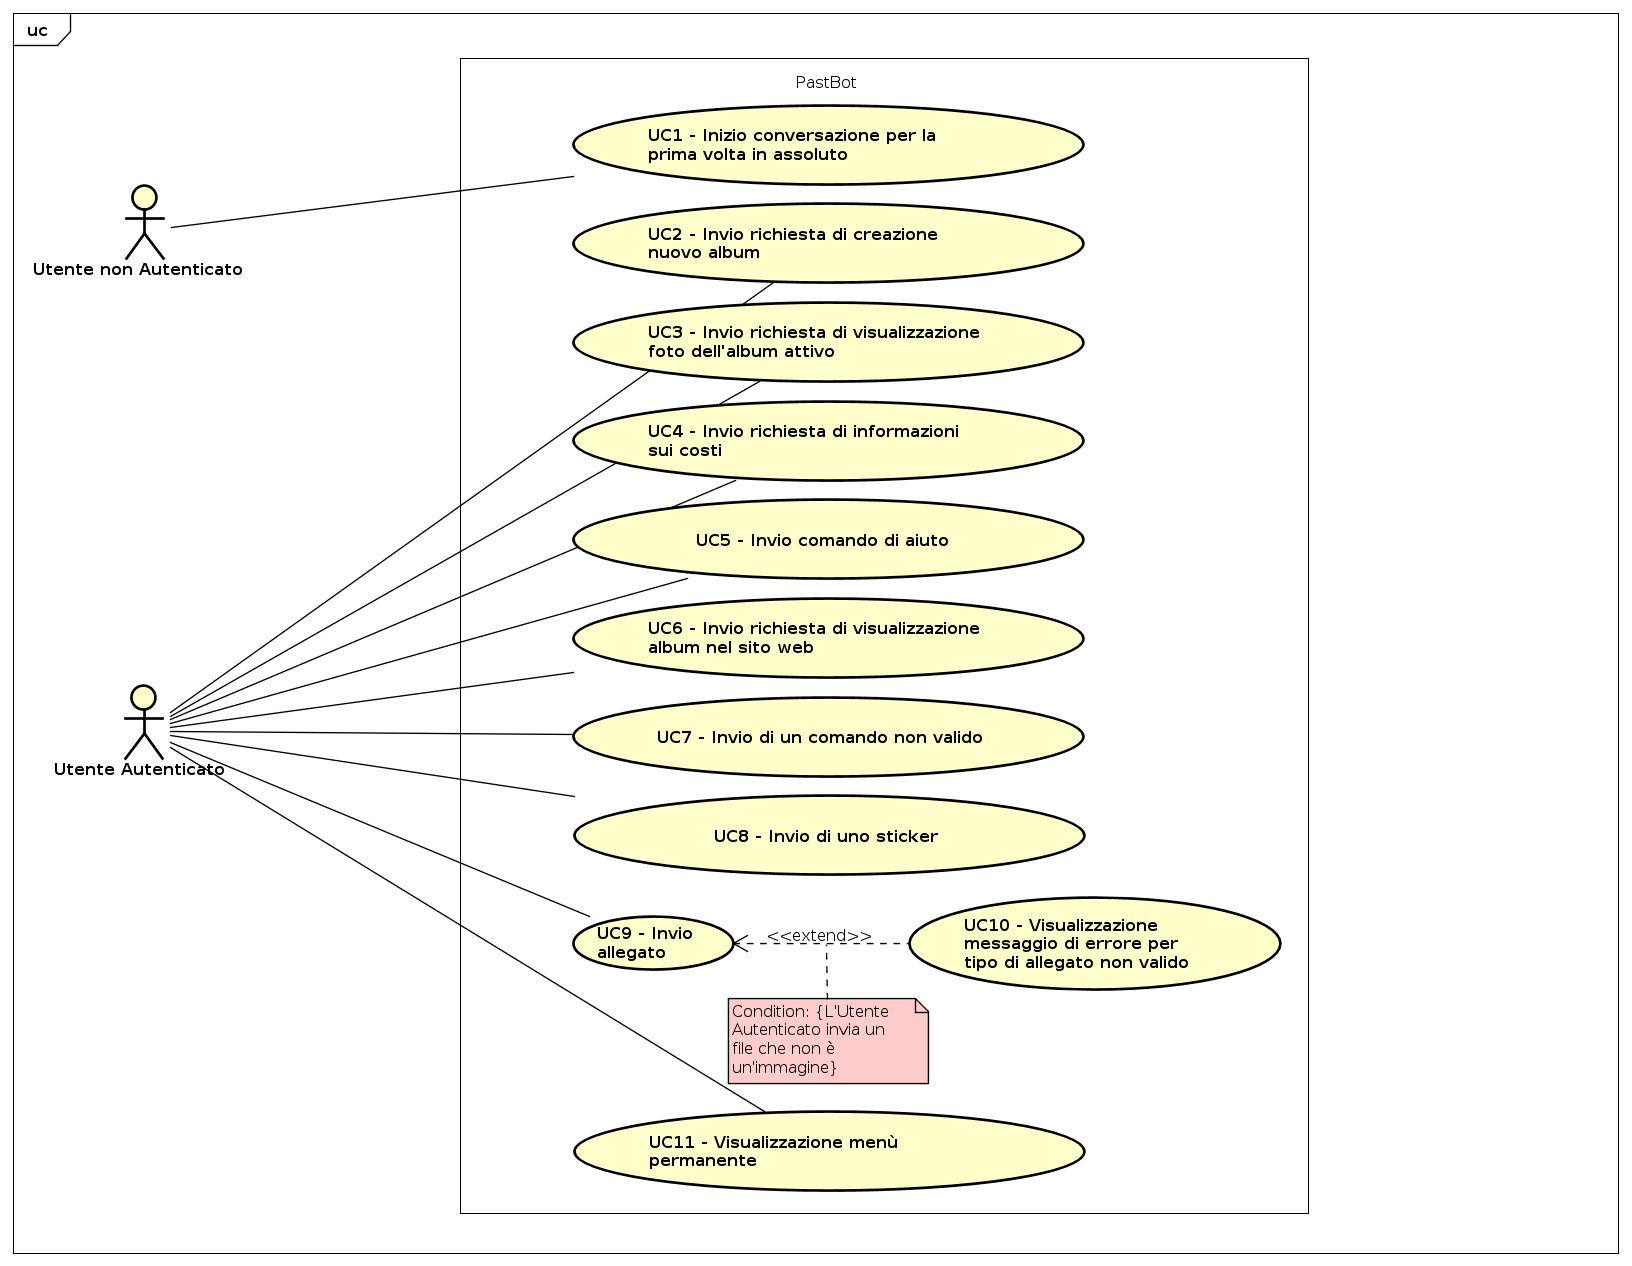
\includegraphics[scale=0.4]{useCase/UC0}
  \caption{Caso d'uso UC0: caso d'uso generale}
\end{figure}

\begin{itemize}
  \item \textbf{Attori}: Utente Non Autenticato, Utente Autenticato;
  \item \textbf{Descrizione}: un utente inanzitutto deve iniziare la
conversazione con il bot. Dopo di che avrà a disposizione il sistema di
conversazione in cui poter mandare messaggi al bot;
  \item \textbf{Precondizione}: l'utente deve aver un account Messenger e deve
averci effettuato la connessione;
  \item \textbf{Postcondizione}: il sistema ha erogato le funzionalità
richieste dall'utente;
  \item \textbf{Flusso principale}:
  \begin{enumerate}
    \item L'Utente Non Autenticato può iniziare una conversazione per la prima
volta in assoluto
    \item L'Utente Autenticato può inviare una richiesta di creazione nuovo
album % FIXME: ref
    \item L'Utente Autenticato può inviare una richiesta visualizzazione album
esistente
    \item L'Utente Autenticato può inviare richiesta informazione sui costi
    \item L'Utente Autenticato può inviare comando di aiuto
    \item L'Utente Autenticato può inviare richiesta di visualizzazione
dell'album nel sito web
    \item L'Utente Autenticato può inviare un comando non valido
    \item L'Utente Autenticato può inviare uno \textit{sticker}
    \item L'Utente Autenticato può inviare un allegato % FIXME: ref
    \item L'Utente Autenticato può visualizzare il menù permanente.
  \end{enumerate}
  \item \textbf{Scenari alternativi}: nessuno.
\end{itemize}

\newpage

\subsection{UC2: invio richiesta di creazione di un nuovo album}
\label{uc:uc2}

\begin{figure}[H]
  \centering
  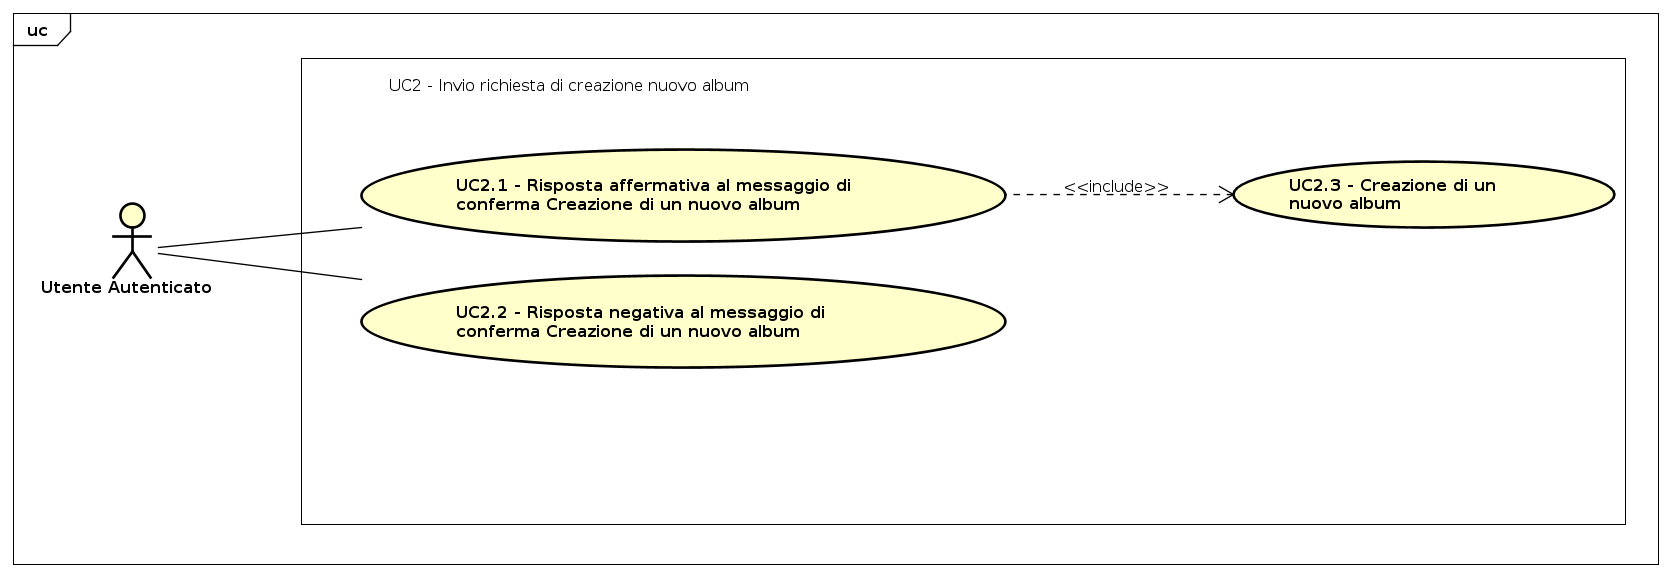
\includegraphics[scale=0.3]{useCase/UC2}
  \caption{UC2: invio richiesta di creazione di un nuovo album}
\end{figure}

\begin{itemize}
  \item \textbf{Attori}: Utente Autenticato;
  \item \textbf{Descrizione}: l'Utente Autenticato procede alla richiesta di
creazione di un nuovo album di foto. Gli verrà posta una domanda per avere
conferma della creazione, alla quale potrà rispondere in maniera affermativa o
negativa
  \item \textbf{Precondizione}: l'Utente Autenticato ha cominciato la
conversazione con il bot
  \item \textbf{Postcondizione}: l'Utente Autenticato ha gestito con successo
il proprio album
  \item \textbf{Flusso principale}:
  \begin{enumerate}
    \item L'Utente Autenticato conferma la creazione di un nuovo album
    \item L'Utente Autenticato non conferma la creazione di un nuovo album
  \end{enumerate}
  \item \textbf{Scenari alternativi}: nessuno.
\end{itemize}


\newpage

\subsection{UC3: invio richiesta di visualizzazione foto dell'album esistente}
\label{uc:uc3}

% FIXME: manca scenario alternativo in UC0.png in cui se viene richiesta una
%lista di un album senza nulla viene segnalato un messaggio di errore.

\begin{figure}[H]
  \centering
  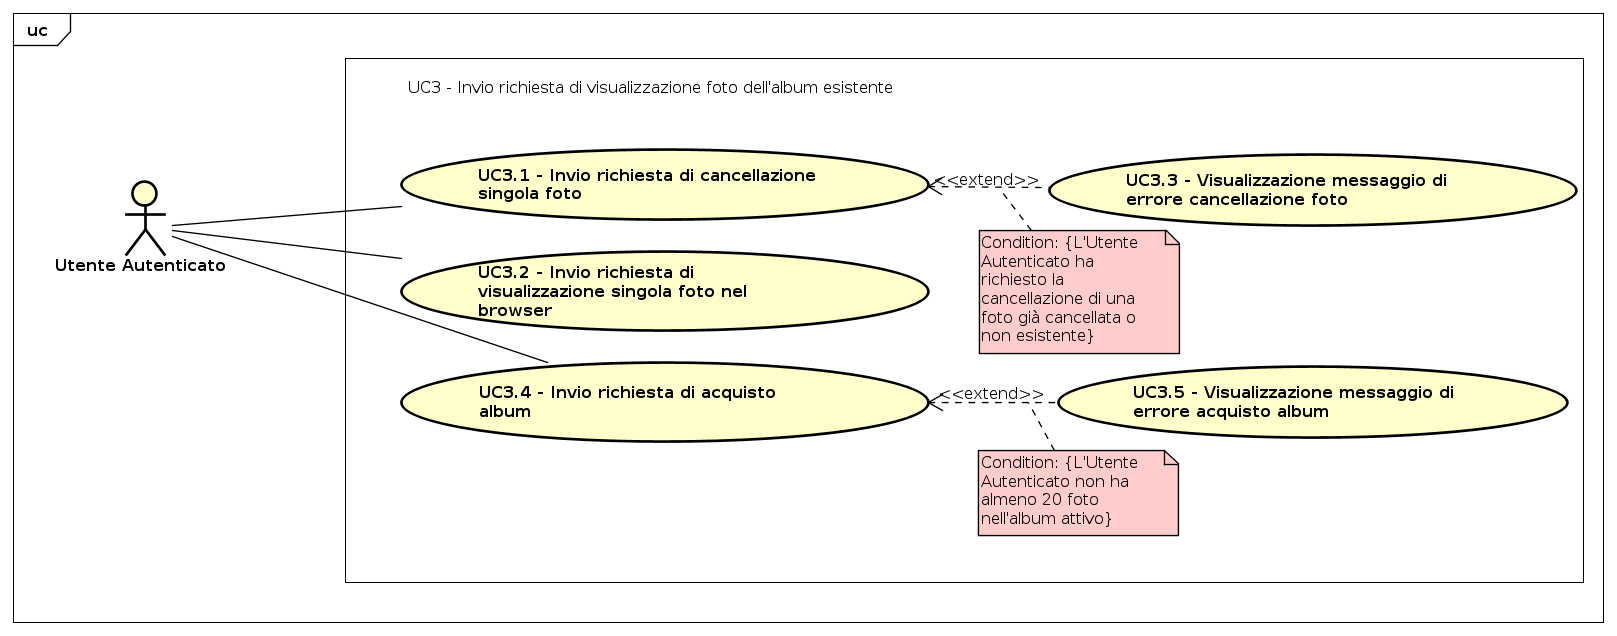
\includegraphics[scale=0.35]{useCase/UC3}
  \caption{UC3: invio richiesta di visualizzazione foto dell'album esistente}
\end{figure}

\begin{itemize}
  \item \textbf{Attori}: Utente Autenticato;
  \item \textbf{Descrizione}: l'Utente può richiedere la visualizzazione della
lista delle foto attualmente caricate, su cui può decidere di cancellarne
alcune, di visualizzarle senza perdita di risoluzione di di acquistarle in un
album.
  \item \textbf{Precondizione}: l'Utente Autenticato ha cominciato la
conversazione con il bot
  \item \textbf{Postcondizione}: l'Utente Autenticato ha visualizzato con
successo la lista delle foto presenti nel proprio album
  \item \textbf{Flusso principale}:
  \begin{enumerate}
    \item L'Utente Autenticato cancella una singola foto dall'album
    \item L'Utente Autenticato visualizza una singola foto dell'album alla
massima risoluzione disponibile
    \item L'Utente Autenticato richiede l'acquisto dell'album
  \end{enumerate}
  \item \textbf{Scenari alternativi}: % FIXME: manca il fatto di un album vuoto
\end{itemize}

\newpage

\subsection{UC11: visualizzazione menù permanente}
\label{uc:uc11}

\begin{figure}[H]
  \centering
  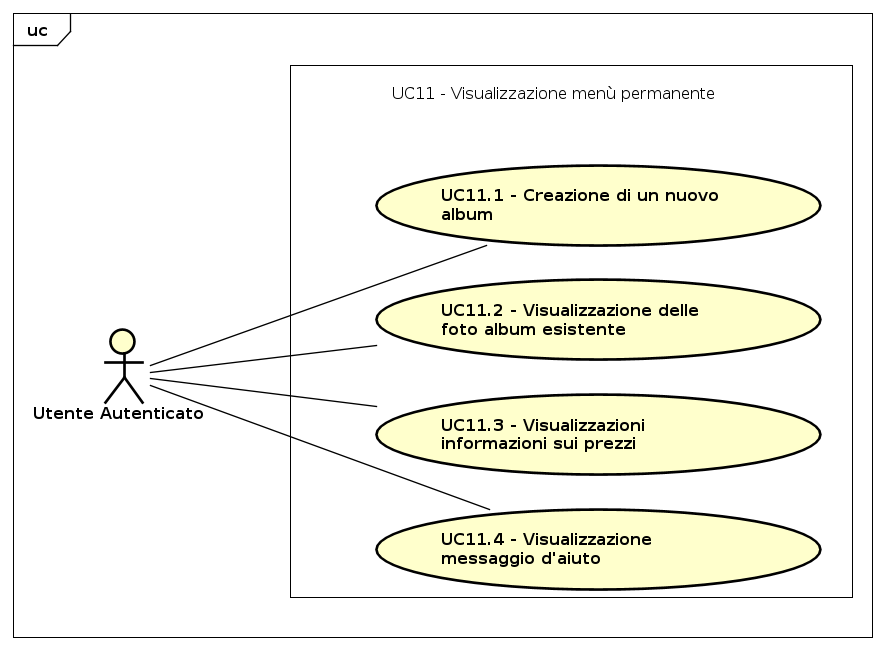
\includegraphics[scale=0.5]{useCase/UC11}
  \caption{UC11: visualizzazione menù permanente}
\end{figure}

\begin{itemize}
  \item \textbf{Attori}: Utente Autenticato;
  \item \textbf{Descrizione}: l'Utente Autenticato ha accesso al menù
permanente con il quale può inviare comandi al bot senza doverli inserire
tramite la tastiera.
  \item \textbf{Precondizione}: l'Utente Autenticato ha cominciato la
conversazione con il bot
  \item \textbf{Postcondizione}: l'Utente Autenticato esegue le operazioni
desiderate con successo
  \item \textbf{Flusso principale}:
  \begin{enumerate}
    \item L'Utente Autenticato effettua la richiesta di creazione di un nuovo
album
    \item L'Utente Autenticato richiede la visualizzazione delle foto esistenti
nell'ultimo album creato
    \item L'Utente Autenticato richiede le informazioni sui prezzi
    \item L'Utente Autenticato richiede la visualizzazione del messaggio di
aiuto
  \end{enumerate}
  \item \textbf{Scenari alternativi}: nessuno
\end{itemize}


% TEMPLATE USECASE
%\newpage
%
%\subsection{UC2: invio richiesta di creazione di un nuovo album}
%\label{uc:uc2}

%\begin{figure}[H]
%  \centering
%  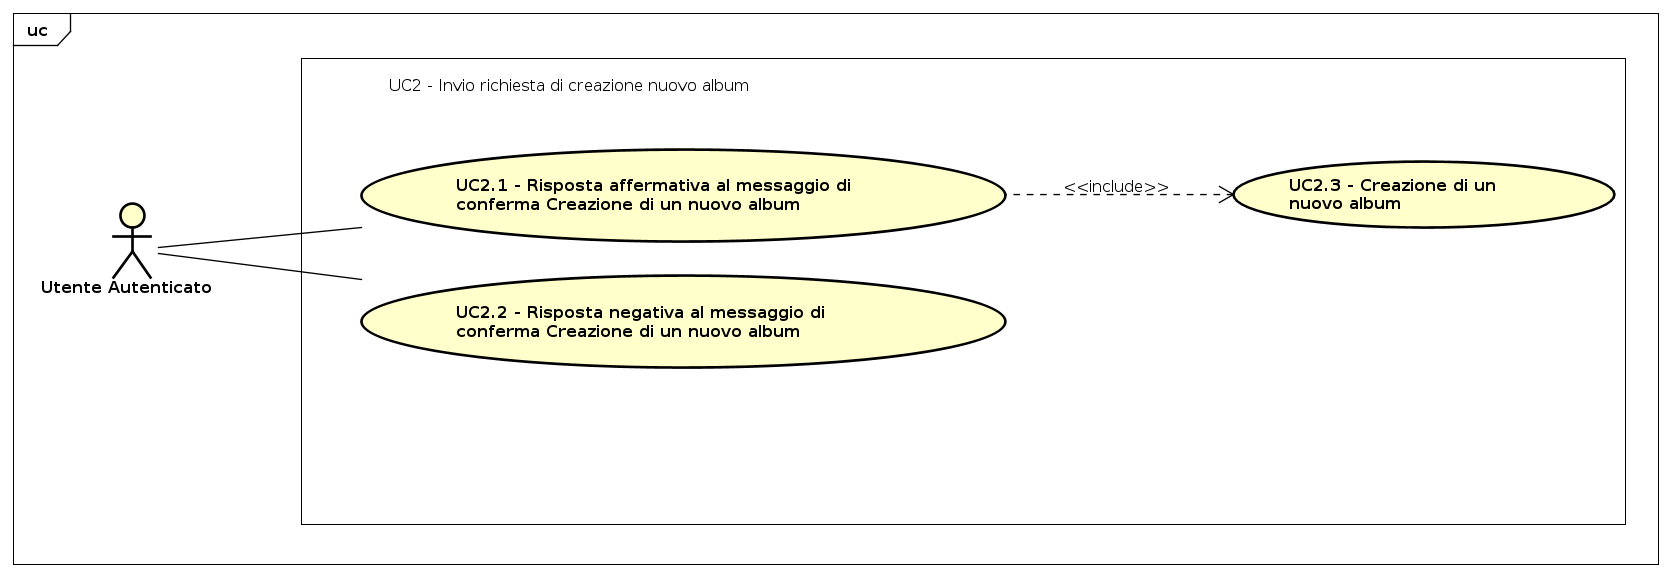
\includegraphics[scale=0.5]{useCase/UC2}
%  \caption{UC2: invio richiesta di creazione di un nuovo album}
%\end{figure}
%
%\begin{itemize}
%  \item \textbf{Attori}: Utente Non Autenticato, Utente Autenticato;
%  \item \textbf{Descrizione}:
%  \item \textbf{Precondizione}:
%  \item \textbf{Postcondizione}:
%  \item \textbf{Flusso principale}:
%  \begin{enumerate}
%    \item
%  \end{enumerate}
%  \item \textbf{Scenari alternativi}:
%\end{itemize}
